\PassOptionsToPackage{quiet}{xeCJK}
\documentclass[answer]{THUExam}
\usepackage{HTNotes-math}
\usepackage{pifont}
\usepackage{ulem}

\usepackage{tikz}
\usetikzlibrary{positioning, calc, shapes.geometric, shapes, shapes.multipart, arrows.meta, arrows, decorations.markings, external, trees}
\usetikzlibrary{patterns, intersections, backgrounds}

% =================================================
%       PDF信息
% =================================================
\title{高等数学A (二)}
\author{}
\Subject{作业}
\Keywords{高等数学, 二重积分, X-型区域, Y-型区域, 积分次序交换}

% =================================================
%       试卷头信息
% =================================================
\Year{2025--2026}
\Semester{春季}
\Course{高等数学A}
\Time{}
\Type{A}

\begin{document}
\vspace{1cm}
\makehead

\vspace{1cm}

% =================================================
%       选择题：二重积分概念与性质
% =================================================
\makepart{选择题}{每小题~4~分，共~12~分}

\begin{problem}
设 $f(x,y)$ 在有界闭区域 $D$ 上连续，则二重积分 $\displaystyle\iint_D f(x,y)\dif\sigma$ 的几何意义是\pickout{C}
\options
{以 $D$ 为底、以曲面 $z=f(x,y)$ 为顶的曲顶柱体的表面积}
{以 $D$ 为边界、以 $z=f(x,y)$ 为高度的柱体侧面积}
{以 $D$ 为底、以曲面 $z=f(x,y)$ 为顶的曲顶柱体的体积（代数和）}
{$f(x,y)$ 在区域 $D$ 上的平均值}
\end{problem}
\begin{note}
当 $f(x,y)\ge 0$ 时，二重积分表示以 $D$ 为底、以曲面 $z=f(x,y)$ 为顶的曲顶柱体的体积。当 $f(x,y)$ 在 $D$ 上变号时，二重积分是各部分体积的代数和——$f\ge 0$ 处取正，$f<0$ 处取负。
\end{note}
\bigskip

\begin{problem}
设 $D=\{(x,y)\mid x^2+y^2\le 1\}$ 为单位圆盘，则 $D$ 作为积分区域\pickout{C}
\options
{仅是 $X$-型区域，不能视为 $Y$-型区域}
{仅是 $Y$-型区域，不能视为 $X$-型区域}
{既可用 $X$-型表示，也可用 $Y$-型表示}
{既非 $X$-型也非 $Y$-型区域}
\end{problem}
\begin{note}
$X$-型：$-1\le x\le 1,\;-\sqrt{1-x^2}\le y\le\sqrt{1-x^2}$；
$Y$-型：$-1\le y\le 1,\;-\sqrt{1-y^2}\le x\le\sqrt{1-y^2}$。
单位圆盘同时满足两种表示。一般地，凸区域通常既是 $X$-型又是 $Y$-型。
\end{note}
\bigskip

\begin{problem}
设 $D$ 由无公共内部的子区域 $D_1$ 与 $D_2$ 拼接而成，$f(x,y)$ 在 $D$ 上可积，则由积分区域可加性有\pickout{B}
\options
{$\displaystyle\iint_D f\dif\sigma = \iint_{D_1} f\dif\sigma \cdot \iint_{D_2} f\dif\sigma$}
{$\displaystyle\iint_D f\dif\sigma = \iint_{D_1} f\dif\sigma + \iint_{D_2} f\dif\sigma$}
{$\displaystyle\iint_D f\dif\sigma = \iint_{D_1} f\dif\sigma - \iint_{D_2} f\dif\sigma$}
{$\displaystyle\iint_D f\dif\sigma = \frac{1}{2}\Bigl(\iint_{D_1} f\dif\sigma + \iint_{D_2} f\dif\sigma\Bigr)$}
\end{problem}
\begin{note}
二重积分的区域可加性：若 $D=D_1\cup D_2$ 且 $D_1\cap D_2$ 的面积为零，则 $\iint_D f\dif\sigma=\iint_{D_1}f\dif\sigma+\iint_{D_2}f\dif\sigma$。这是将复杂区域拆分为简单子区域计算的理论基础。
\end{note}
\bigskip

% =================================================
%       填空题：交换积分次序
% =================================================
\newpage
\makepart{填空题}{每小题~6~分，共~12~分}

\begin{problem}
交换积分次序：$\displaystyle\int_0^1\dif x\int_{x^2}^x f(x,y)\dif y ={}$\fillin{$\displaystyle\int_0^1\dif y\int_y^{\sqrt{y}}f(x,y)\dif x$}.
\end{problem}
\begin{note}
积分区域 $D$ 由下边界 $y=x^2$ 和上边界 $y=x$ 在 $x\in[0,1]$ 上围成。

\begin{center}
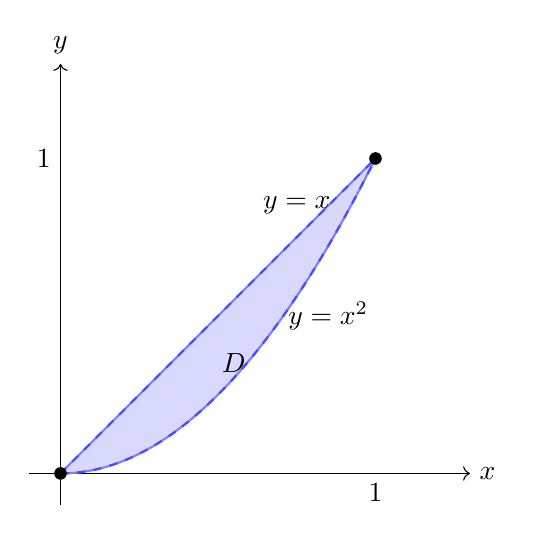
\begin{tikzpicture}[scale=4]
    \draw[->] (-0.1,0) -- (1.3,0) node[right] {$x$};
    \draw[->] (0,-0.1) -- (0,1.3) node[above] {$y$};
    \fill[blue!15, draw=blue!50, thick]
        (0,0) -- plot[domain=0:1, samples=100] (\x, \x) --
        plot[domain=1:0, samples=100] (\x, \x*\x) -- cycle;
    \draw[blue!70, thick, dashed, domain=0:1, samples=100] plot (\x, \x);
    \draw[blue!70, thick, dashed, domain=0:1, samples=100] plot (\x, \x*\x);
    \node[below] at (1,0) {$1$};
    \node[left] at (0,1) {$1$};
    \node at (0.55,0.35) {$D$};
    \node at (0.75,0.85) {$y=x$};
    \node at (0.85,0.5) {$y=x^2$};
    \fill (0,0) circle (0.02);
    \fill (1,1) circle (0.02);
\end{tikzpicture}
\end{center}

改写为 $Y$-型：对固定的 $y\in[0,1]$，$x$ 的左边界为 $x=y$（来自 $y=x$），右边界为 $x=\sqrt{y}$（来自 $y=x^2$），且 $\sqrt{y}\ge y$ 在 $[0,1]$ 上成立。
\end{note}
\bigskip

\begin{problem}
交换积分次序：$\displaystyle\int_0^2\dif x\int_{x/2}^1 f(x,y)\dif y ={}$\fillin{$\displaystyle\int_0^1\dif y\int_0^{2y}f(x,y)\dif x$}.
\end{problem}
\begin{note}
积分区域 $D$ 由下边界 $y=x/2$ 和上边界 $y=1$ 围成，$x\in[0,2]$。

\begin{center}
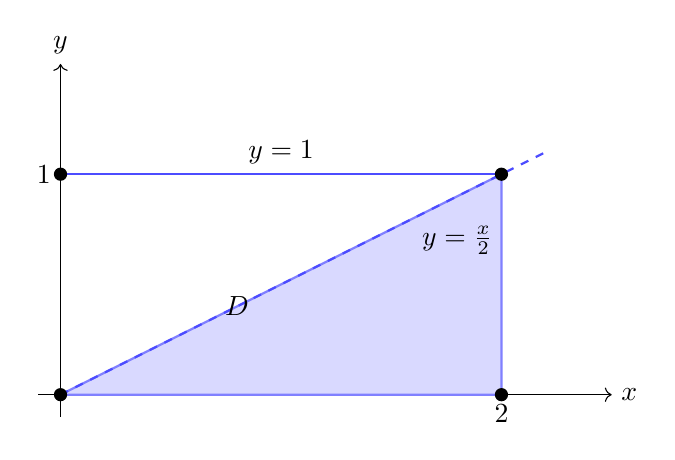
\begin{tikzpicture}[scale=2.8]
    \draw[->] (-0.1,0) -- (2.5,0) node[right] {$x$};
    \draw[->] (0,-0.1) -- (0,1.5) node[above] {$y$};
    \fill[blue!15, draw=blue!50, thick]
        (0,0) -- (2,1) -- (2,0) -- cycle;
    \draw[blue!70, thick, dashed] (0,0) -- (2.2,1.1);
    \draw[blue!70, thick] (0,1) -- (2,1);
    \node[below] at (2,0) {$2$};
    \node[left] at (0,1) {$1$};
    \node at (0.8,0.4) {$D$};
    \node at (1.8,0.7) {$y=\frac{x}{2}$};
    \node at (1,1.1) {$y=1$};
    \fill (0,0) circle (0.03);
    \fill (2,0) circle (0.03);
    \fill (2,1) circle (0.03);
    \fill (0,1) circle (0.03);
\end{tikzpicture}
\end{center}

改写为 $Y$-型：$y\in[0,1]$，对固定的 $y$，左边界为 $x=0$，右边界为 $x=2y$（来自 $y=x/2$）。
\end{note}
\bigskip

% =================================================
%       计算题
% =================================================
\newpage
\makepart{计算题}{第1小题~11~分，第2、3小题各~12~分，共~35~分}

\begin{problem}
计算二重积分 $\displaystyle I=\iint_D (x+y)\dif\sigma$，其中 $D$ 是由直线 $x=0,\ y=0,\ x+y=1$ 围成的三角形闭区域。
\end{problem}
\begin{note}
将 $D$ 视为 $X$-型区域：$0\le x\le 1,\;0\le y\le 1-x$。这是标准的直角三角形区域，三条边界均为直线段。

\begin{center}
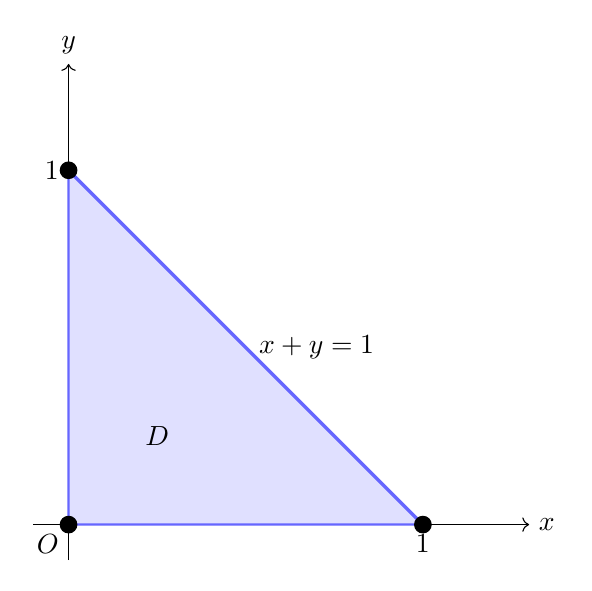
\begin{tikzpicture}[scale=4.5]
    \draw[->] (-0.1,0) -- (1.3,0) node[right] {$x$};
    \draw[->] (0,-0.1) -- (0,1.3) node[above] {$y$};
    \fill[blue!12, draw=blue!60, thick]
        (0,0) -- (1,0) -- (0,1) -- cycle;
    \draw[blue!60, very thick] (1,0) -- (0,1);
    \node[below] at (1,0) {$1$};
    \node[left] at (0,1) {$1$};
    \node at (0.25,0.25) {$D$};
    \node at (0.7,0.5) {$x+y=1$};
    \node[below left] at (0,0) {$O$};
    \fill (0,0) circle (0.025);
    \fill (1,0) circle (0.025);
    \fill (0,1) circle (0.025);
\end{tikzpicture}
\end{center}
\end{note}
\begin{solution}
将积分区域 $D$ 视为 $X$-型区域：
\[
D=\{(x,y)\mid 0\le x\le 1,\; 0\le y\le 1-x\}.
\]
于是
\begin{align*}
I &= \int_0^1\dif x\int_0^{1-x}(x+y)\dif y
   = \int_0^1 \Bigl[xy+\frac{y^2}{2}\Bigr]_{y=0}^{y=1-x}\dif x \\[4pt]
  &= \int_0^1 \Bigl(x(1-x)+\frac{(1-x)^2}{2}\Bigr)\dif x
   = \int_0^1 \Bigl(x-x^2+\frac{1-2x+x^2}{2}\Bigr)\dif x \\[4pt]
  &= \int_0^1 \Bigl(\frac{1}{2}-\frac{x^2}{2}\Bigr)\dif x
   = \Bigl[\frac{x}{2}-\frac{x^3}{6}\Bigr]_0^1
   = \frac{1}{2}-\frac{1}{6}
   = \boxed{\dfrac{1}{3}}.
\end{align*}
\textbf{解法二（$Y$-型区域）：} 将 $D$ 视为 $Y$-型区域，
\[
D=\{(x,y)\mid 0\le y\le 1,\; 0\le x\le 1-y\}.
\]
则
\begin{align*}
I &= \int_0^1\dif y\int_0^{1-y}(x+y)\dif x
   = \int_0^1 \Bigl[\frac{x^2}{2}+yx\Bigr]_{x=0}^{x=1-y}\dif y \\[4pt]
  &= \int_0^1 \Bigl(\frac{(1-y)^2}{2}+y(1-y)\Bigr)\dif y
   = \int_0^1 \Bigl(\frac{1-2y+y^2}{2}+y-y^2\Bigr)\dif y \\[4pt]
  &= \int_0^1 \Bigl(\frac{1}{2}-\frac{y^2}{2}\Bigr)\dif y
   = \Bigl[\frac{y}{2}-\frac{y^3}{6}\Bigr]_0^1
   = \frac{1}{2}-\frac{1}{6}
   = \boxed{\dfrac{1}{3}}.
\end{align*}
该区域既是 $X$-型又是 $Y$-型，被积函数关于 $x,y$ 对称，两种次序计算量相当。
\end{solution}


\vspace{0.8cm}

\begin{problem}
计算二重积分 $\displaystyle I=\iint_D \mathrm{e}^{y^2}\dif\sigma$，其中 $D$ 是由直线 $y=x$，$y=1$ 及 $y$ 轴（$x=0$）围成的三角形闭区域。
\end{problem}
\begin{note}
本题的难点在于被积函数 $\mathrm{e}^{y^2}$ 对 $y$ 没有初等原函数。若将 $D$ 视为 $X$-型区域（先 $y$ 后 $x$），内层积分 $\int_x^1\mathrm{e}^{y^2}\dif y$ 无法用初等函数表示。但若将 $D$ 视为 $Y$-型区域（先 $x$ 后 $y$），被积函数对 $x$ 仅为常数，内层积分极其简单，外层恰可通过凑微分求解。

\begin{center}
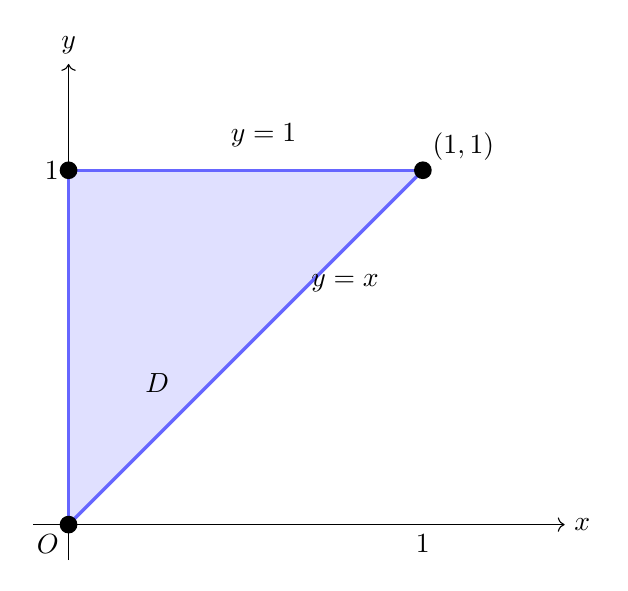
\begin{tikzpicture}[scale=4.5]
    \draw[->] (-0.1,0) -- (1.4,0) node[right] {$x$};
    \draw[->] (0,-0.1) -- (0,1.3) node[above] {$y$};

    % Filled region: triangle (0,0)-(1,1)-(0,1)
    \fill[blue!12, draw=blue!60, thick]
        (0,0) -- (1,1) -- (0,1) -- cycle;

    % Boundary curves
    \draw[blue!60, very thick] (0,1) -- (1,1);
    \draw[blue!60, very thick] (0,0) -- (1,1);
    \draw[blue!60, very thick] (0,0) -- (0,1);

    \node[below] at (1,0) {$1$};
    \node[left] at (0,1) {$1$};
    \node at (0.25,0.4) {$D$};
    \node at (0.78,0.68) {$y=x$};
    \node at (0.55,1.1) {$y=1$};
    \node[below left] at (0,0) {$O$};
    \fill (0,0) circle (0.025);
    \fill (1,1) circle (0.025);
    \fill (0,1) circle (0.025);
    \node[above right] at (1,1) {$(1,1)$};
\end{tikzpicture}
\end{center}
\end{note}
\begin{solution}
\textbf{分析两种积分次序：}
\begin{itemize}
    \item 若按 $X$-型：$D=\{(x,y)\mid 0\le x\le 1,\;x\le y\le 1\}$，则
    \[
    I = \int_0^1\dif x\int_x^1\mathrm{e}^{y^2}\dif y,
    \]
    内层积分 $\int\mathrm{e}^{y^2}\dif y$ 没有初等原函数，无法继续。
    \item 若按 $Y$-型：$D=\{(x,y)\mid 0\le y\le 1,\;0\le x\le y\}$，则
    \begin{align*}
    I &= \int_0^1\dif y\int_0^y\mathrm{e}^{y^2}\dif x
       = \int_0^1 \mathrm{e}^{y^2}\Bigl[x\Bigr]_{x=0}^{x=y}\dif y
       = \int_0^1 y\,\mathrm{e}^{y^2}\dif y.
    \end{align*}
    令 $u=y^2$，则 $\dif u=2y\dif y$，即 $y\dif y=\frac{1}{2}\dif u$。当 $y=0$ 时 $u=0$，当 $y=1$ 时 $u=1$，于是
    \[
    I = \int_0^1 \mathrm{e}^{u}\cdot\frac{1}{2}\dif u
       = \frac{1}{2}\Bigl[\mathrm{e}^{u}\Bigr]_0^1
       = \boxed{\dfrac{\mathrm{e}-1}{2}}.
    \]
\end{itemize}
\end{solution}


\newpage

\begin{problem}
计算二重积分 $\displaystyle I=\iint_D y\dif\sigma$，其中 $D$ 是由曲线 $y=\sqrt{x}$，直线 $y=0$ 和 $x+y=2$ 围成的在第一象限内的有界闭区域。
\end{problem}
\begin{note}
若将 $D$ 视为 $X$-型区域，则需要以 $x=1$ 为界拆分为 $D_1$ 和 $D_2$ 两个子区域分别积分（左侧上边界为 $y=\sqrt{x}$，右侧上边界为 $y=2-x$）。若将 $D$ 视为 $Y$-型区域，则无需拆分，一次积分即可完成。

先求关键交点：$y=\sqrt{x}$ 与 $x+y=2$ 联立，消去 $x$ 得 $y^2+y-2=0$，解得 $y=1$（负根舍去），对应 $x=1$，即交点为 $(1,1)$。

\begin{center}
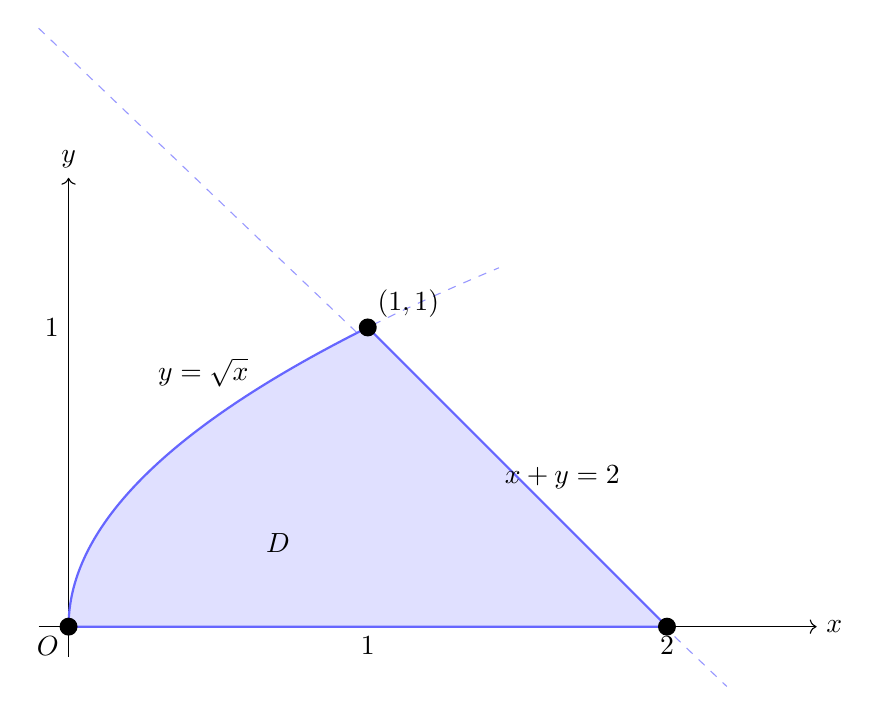
\begin{tikzpicture}[scale=3.8]
    % Axes
    \draw[->] (-0.1,0) -- (2.5,0) node[right] {$x$};
    \draw[->] (0,-0.1) -- (0,1.5) node[above] {$y$};

    % Dashed full curves for context
    \draw[blue!40, dashed, domain=0:1.2, samples=80] plot (\x*\x, \x);
    \draw[blue!40, dashed] (-0.1,2) -- (2.2,-0.2);

    % Filled region D
    \fill[blue!12, draw=blue!60, thick]
        (0,0) -- plot[domain=0:1, samples=80] (\x*\x, \x) --
        plot[domain=1:2, samples=80] (\x, {2-\x}) -- (2,0) -- cycle;

    \node[below] at (1,0) {$1$};
    \node[below] at (2,0) {$2$};
    \node[left] at (0,1) {$1$};
    \node at (0.7,0.28) {$D$};
    \node at (0.45,0.85) {$y=\sqrt{x}$};
    \node at (1.65,0.5) {$x+y=2$};
    \node[below left] at (0,0) {$O$};

    \fill (0,0) circle (0.03);
    \fill (1,1) circle (0.03);
    \fill (2,0) circle (0.03);
    \node[above right] at (1,1) {$(1,1)$};
\end{tikzpicture}
\end{center}
\end{note}
\begin{solution}
将 $D$ 视为 $Y$-型区域，$D=\{(x,y)\mid 0\le y\le 1,\; y^2\le x\le 2-y\}$，无需拆分：
\begin{align*}
I &= \int_0^1\dif y\int_{y^2}^{2-y} y\dif x
   = \int_0^1 y\Bigl[x\Bigr]_{x=y^2}^{x=2-y}\dif y
   = \int_0^1 y\bigl((2-y)-y^2\bigr)\dif y \\[4pt]
  &= \int_0^1 (2y-y^2-y^3)\dif y
   = \Bigl[y^2-\frac{y^3}{3}-\frac{y^4}{4}\Bigr]_0^1 \\[4pt]
  &= 1-\frac{1}{3}-\frac{1}{4}
   = \frac{12}{12}-\frac{4}{12}-\frac{3}{12}
   = \boxed{\dfrac{5}{12}}.
\end{align*}

（若按 $X$-型拆分计算：
$D_1=\{(x,y)\mid 0\le x\le 1,\;0\le y\le\sqrt{x}\}$，
$D_2=\{(x,y)\mid 1\le x\le 2,\;0\le y\le 2-x\}$，
需要分别计算 $\iint_{D_1}y\dif\sigma$ 和 $\iint_{D_2}y\dif\sigma$ 再相加，过程明显冗长。）
\end{solution}

\end{document}
